\documentclass[a4paper,11pt]{article}
\usepackage[dvipsnames,table]{xcolor}
\usepackage[a4paper,margin=2.5cm,headheight=15pt]{geometry}
\usepackage[utf8]{inputenc}
\usepackage[T1]{fontenc}
\usepackage[serbian]{babel}
\usepackage{lmodern,microtype}
\usepackage{amsmath,amssymb,mathtools}
\numberwithin{equation}{section}
\usepackage{graphicx,adjustbox,placeins,needspace}
\graphicspath{{Images/}}
\usepackage{booktabs,tabularx,longtable,array,multirow,makecell}
\usepackage{caption,subcaption}
\captionsetup{font=small,labelfont=bf}
\usepackage{siunitx}
\sisetup{detect-all}
\usepackage[most]{tcolorbox}
\usetikzlibrary{tikzmark,arrows.meta,calc}
\usepackage{enumitem}
\setlist{nosep}
\usepackage{fancyhdr}
\definecolor{Primary}{HTML}{1F77B4}
\definecolor{Accent}{HTML}{2CA02C}
\usepackage[colorlinks=true,linkcolor=Primary,citecolor=Primary,urlcolor=Primary]{hyperref}
\usepackage{cleveref}
\pagestyle{fancy}
\fancyhf{}
\lhead{\small\textit{Kodovi}}
\rhead{\thepage}
\renewcommand{\arraystretch}{1.25}
\newcolumntype{C}{>{\centering\arraybackslash}X}
\renewcommand{\contentsname}{Sadržaj}
\setlength{\emergencystretch}{2em}
\allowdisplaybreaks[2]
\newcommand{\napomena}[1]{\begin{tcolorbox}[colback=gray!10,colframe=black,boxrule=0.5pt,breakable]#1\end{tcolorbox}}
\newcommand{\redlinija}{\arrayrulecolor{black!28}\specialrule{0.3pt}{2pt}{2pt}\arrayrulecolor{black}}
\newcommand{\kod}[1]{\ensuremath{\mathtt{#1}}}
\newcommand{\istaknutbit}[1]{\textcolor{Primary!85!black}{\ifmmode\mathbf{#1}\else\textbf{#1}\fi}}
\begin{document}
\hypersetup{pageanchor=false}
\begin{titlepage}
\thispagestyle{empty}
\begin{center}
{\Large\bfseries UNIVERZITET U BEOGRADU -- ELEKTROTEHNIČKI FAKULTET\\ KATEDRA ZA ELEKTRONIKU\par}
\vspace{25mm}
{\LARGE\bfseries DIGITALNA ELEKTRONIKA 1\par}
\vspace{2mm}
{\large Materijali za računske vežbe\par}
\vspace{18mm}
{\Large\bfseries KODOVI\par}
\vspace{3mm}
{\large Vežbe 5\par}
\vfill
\begin{minipage}{0.62\linewidth}
\raggedright\textbf{Autori:}\\[4pt]\small
\begin{tabular}{@{}ll@{}}
Nikola Petrović & \href{mailto:p.z.nikola@etf.bg.ac.rs}{\texttt{p.z.nikola@etf.bg.ac.rs}}\\
Haris Turkmanović & \href{mailto:haris@etf.bg.ac.rs}{\texttt{haris@etf.bg.ac.rs}}\\
\end{tabular}
\end{minipage}\hfill
\begin{minipage}{0.34\linewidth}\raggedleft Beograd, \today\end{minipage}
\end{center}
\end{titlepage}
\hypersetup{pageanchor=true}
\tableofcontents
\newpage

% Izvor DOCX: blok 22
\FloatBarrier
\section{Uvod}\label{sec:1}


% Izvor DOCX: blok 23
\FloatBarrier
\subsection{Kodovi}\label{sec:1.1}


% Izvor DOCX: blok 24
U digitalnim sistemima se mogu koristiti različiti kodovi za predstavljanje decimalnih brojeva. U ovim vežbama razmatramo sledeće vrste kodova. To nije podela na međusobno isključive grupe: svojstvo detekcije greške može imati i težinski, netežinski ili alfanumerički kod.



% Izvor DOCX: blok 25
\begin{itemize}[leftmargin=*]
\item Težinski binarni kodovi

\item Netežinski binarni kodovi

\item Alfanumerički kodovi

\item Kodovi sa mogućnošću detekcije greške

\end{itemize}


% Izvor DOCX: blok 26
U okviru računskih vežbi obrađivaćemo bar jedan od kodova iz svake od grupa, osim alfanumeričkih.



% Izvor DOCX: blok 27
\subsubsection{Težinski kodovi}\label{sec:1.1.1}


% Izvor DOCX: blok 28
\Needspace{6\baselineskip}
\textbf{BCD8421}



% Izvor DOCX: blok 29
BCD8421 (skraćeno BCD) svaku decimalnu cifru predstavlja sa četiri bita, težina 8, 4, 2 i 1, redom od najvišeg bita. Tabela~\ref{tab:bcd} prikazuje dozvoljene kodne reči; preostalih šest četvorobitnih kombinacija nije dozvoljeno.

% Izvor DOCX: blok 30
\begin{table}[!htbp]\centering\caption{Kod BCD8421.}\label{tab:bcd}
\begin{adjustbox}{max width=\linewidth}\begin{tabular}{cc}\toprule
Cifra & Kodna reč\\\midrule
0 & $\mathtt{0000}$\\
\redlinija
1 & $\mathtt{0001}$\\
\redlinija
2 & $\mathtt{0010}$\\
\redlinija
3 & $\mathtt{0011}$\\
\redlinija
4 & $\mathtt{0100}$\\
\redlinija
5 & $\mathtt{0101}$\\
\redlinija
6 & $\mathtt{0110}$\\
\redlinija
7 & $\mathtt{0111}$\\
\redlinija
8 & $\mathtt{1000}$\\
\redlinija
9 & $\mathtt{1001}$\\
\bottomrule\end{tabular}\end{adjustbox}
\end{table}


% Izvor DOCX: blok 31


% Izvor DOCX: blok 32
Za kodovanje decimalnog broja svaka cifra se zasebno zamenjuje četvorobitnom reči iz tabele~\ref{tab:bcd}.

% Izvor DOCX: blok 33
\Needspace{6\baselineskip}
\textbf{BCD2421}



% Izvor DOCX: blok 34
Kod BCD2421 takođe koristi četiri bita po decimalnoj cifri, ali njihove težine su 2, 4, 2 i 1. Izbor kodnih reči u tabeli~\ref{tab:2421} čini kod samokomplementarnim.

% Izvor DOCX: blok 35
\begin{table}[!htbp]\centering
\caption{Kod BCD2421: komplementarnost u odnosu na horizontalnu osu između cifara 4 i 5.}\label{tab:2421}
\begin{tabular}{ccc}\toprule
Cifra $d$ & Kodna reč $c(d)$ & Uparena cifra $9-d$\\
\midrule
\rowcolor{blue!7}0 & $\mathtt{0000}$ & $9$ \\
\redlinija
\rowcolor{green!8}1 & $\mathtt{0001}$ & $8$ \\
\redlinija
\rowcolor{orange!9}2 & $\mathtt{0010}$ & $7$ \\
\redlinija
\rowcolor{violet!7}3 & $\mathtt{0011}$ & $6$ \\
\redlinija
\rowcolor{cyan!9}4 & $\mathtt{0100}$ & $5$ \\
\arrayrulecolor{red!70!black}\specialrule{.8pt}{2pt}{2pt}\arrayrulecolor{black}
\rowcolor{cyan!9}5 & $\mathtt{1011}$ & $4$ \\
\redlinija
\rowcolor{violet!7}6 & $\mathtt{1100}$ & $3$ \\
\redlinija
\rowcolor{orange!9}7 & $\mathtt{1101}$ & $2$ \\
\redlinija
\rowcolor{green!8}8 & $\mathtt{1110}$ & $1$ \\
\redlinija
\rowcolor{blue!7}9 & $\mathtt{1111}$ & $0$ \\
\bottomrule\end{tabular}
\par\smallskip\small Jednako obojeni redovi čine par; crvena linija označava osu.
\end{table}

% Izvor DOCX: blok 36


% Izvor DOCX: blok 37
Jednako obojeni redovi u tabeli~\ref{tab:2421} nalaze se na jednakom rastojanju od crvene horizontalne ose. Njihove kodne reči su bit po bit komplementarne: $c(9-d)=\overline{c(d)}$. Parovi su $0\leftrightarrow9$, $1\leftrightarrow8$, $2\leftrightarrow7$, $3\leftrightarrow6$, $4\leftrightarrow5$. To je antisimetrija vrednosti bita ($0\leftrightarrow1$), odnosno samokomplementarnost koda. Za cifre 0–4 kod se poklapa sa BCD8421.

% Izvor DOCX: blok 38
\FloatBarrier\Needspace{7\baselineskip}
\subsubsection{Netežinski kodovi}\label{sec:1.1.2}


% Izvor DOCX: blok 39
\Needspace{6\baselineskip}
\textbf{Više 3}



% Izvor DOCX: blok 40
Kod „više 3“ je netežinski kod. Svaka decimalna cifra $d$ koduje se četvorobitnim binarnim zapisom broja $d+3$, prema tabeli~\ref{tab:excess}.

% Izvor DOCX: blok 41


% Izvor DOCX: blok 42
\begin{table}[!htbp]\centering\caption{Kod „više 3“.}\label{tab:excess}
\begin{adjustbox}{max width=\linewidth}\begin{tabular}{cc}\toprule
Cifra & Kodna reč\\\midrule
0 & $\mathtt{0011}$\\
\redlinija
1 & $\mathtt{0100}$\\
\redlinija
2 & $\mathtt{0101}$\\
\redlinija
3 & $\mathtt{0110}$\\
\redlinija
4 & $\mathtt{0111}$\\
\redlinija
5 & $\mathtt{1000}$\\
\redlinija
6 & $\mathtt{1001}$\\
\redlinija
7 & $\mathtt{1010}$\\
\redlinija
8 & $\mathtt{1011}$\\
\redlinija
9 & $\mathtt{1100}$\\
\bottomrule\end{tabular}\end{adjustbox}
\end{table}


% Izvor DOCX: blok 43
Kod je samokomplementaran: $15-(d+3)=(9-d)+3$. Pri dekodiranju se od binarne vrednosti svake dozvoljene četvorobitne reči oduzima 3.

% Izvor DOCX: blok 44
\Needspace{6\baselineskip}
\textbf{Binarni Grejov kod}



% Izvor DOCX: blok 45
Reflektovani binarni Grejov kod predstavlja cele nenegativne brojeve zadate širine. Uzastopne kodne reči razlikuju se u tačno jednom bitu. To smanjuje neodređenost očitavanja pri prelazu između susednih vrednosti; ne garantuje odsustvo svih gličeva u proizvoljnoj kombinacionoj mreži.

% Izvor DOCX: blok 46
Postoje dva pristupa za određivanje kodne reči:



% Izvor DOCX: blok 47
Prvi pristup je reflektovana konstrukcija:


% Izvor DOCX: blok 48
\begin{enumerate}[label=\arabic*.,start=1,leftmargin=*]
\item Odredi se potrebna dužina kodne reči \emph{n} za predstavu brojeva

\item Ukoliko je $n=1$, broju 0 odgovara Grejova kodna reč 0, a broju 1 kodna reč 1.

\item Ukoliko je dužina kodne reči veća od 1, kodne reči dužine \emph{n} dobijamo iterativnim postupkom koji podrazumeva postepeno određivanje kodnih reči dužine 2, 3 \ldots{} sve do \emph{n} i to tako što:

\begin{enumerate}[label=\arabic*.,start=1,leftmargin=*]
\item prva polovina, koja sadrži $2^{n-1}$ kodnih reči, dobija se tako što se za krajnji levi bit uzme 0 dok preostali biti predstavljaju kodne reči Grejovog koda dužine $n-1$.

\item druga polovina, koja sadrži $2^{n-1}$ kodnih reči, dobija se tako što se za krajnji levi bit uzme 1 dok preostali biti predstavljaju kodne reči Grejovog koda dužine $n-1$ zapisane u obrnutom poretku.

\end{enumerate}
\end{enumerate}


% Izvor DOCX: blok 49
Tabela~\ref{tab:graybuild} prikazuje sve korake do širine $n=4$.


% Izvor DOCX: blok 50
\begin{table}[!htbp]\centering\caption{Reflektovana konstrukcija Grejovog koda od jednog do četiri bita.}\label{tab:graybuild}
\begin{minipage}[t]{.24\linewidth}\centering$n=1$

\begin{tabular}{cc}\toprule
$i$ & $g_0$\\
\midrule
0 & \texttt{0}\\
\redlinija
1 & \texttt{1}\\
\bottomrule\end{tabular}
\end{minipage}\hfill
\begin{minipage}[t]{.24\linewidth}\centering$n=2$

\setlength{\tabcolsep}{3pt}\begin{tabular}{cccc}\toprule
$i$ & $g_{1}$ & $g_0$ & red\\
\midrule
0 & \textcolor{Primary}{\texttt{0}} & \cellcolor{blue!8}\texttt{0} & $\downarrow$\\
\redlinija
1 & \textcolor{Primary}{\texttt{0}} & \cellcolor{blue!8}\texttt{1} & $\downarrow$\\
\arrayrulecolor{red!70!black}\specialrule{.6pt}{2pt}{2pt}\arrayrulecolor{black}
2 & \textcolor{Primary}{\texttt{1}} & \cellcolor{orange!12}\texttt{1} & $\uparrow$\\
\redlinija
3 & \textcolor{Primary}{\texttt{1}} & \cellcolor{orange!12}\texttt{0} & $\uparrow$\\
\bottomrule\end{tabular}
\end{minipage}\hfill
\begin{minipage}[t]{.24\linewidth}\centering$n=3$

\setlength{\tabcolsep}{3pt}\begin{tabular}{cccc}\toprule
$i$ & $g_{2}$ & $g_{1}\dots g_0$ & red\\
\midrule
0 & \textcolor{Primary}{\texttt{0}} & \cellcolor{blue!8}\texttt{00} & $\downarrow$\\
\redlinija
1 & \textcolor{Primary}{\texttt{0}} & \cellcolor{blue!8}\texttt{01} & $\downarrow$\\
\redlinija
2 & \textcolor{Primary}{\texttt{0}} & \cellcolor{blue!8}\texttt{11} & $\downarrow$\\
\redlinija
3 & \textcolor{Primary}{\texttt{0}} & \cellcolor{blue!8}\texttt{10} & $\downarrow$\\
\arrayrulecolor{red!70!black}\specialrule{.6pt}{2pt}{2pt}\arrayrulecolor{black}
4 & \textcolor{Primary}{\texttt{1}} & \cellcolor{orange!12}\texttt{10} & $\uparrow$\\
\redlinija
5 & \textcolor{Primary}{\texttt{1}} & \cellcolor{orange!12}\texttt{11} & $\uparrow$\\
\redlinija
6 & \textcolor{Primary}{\texttt{1}} & \cellcolor{orange!12}\texttt{01} & $\uparrow$\\
\redlinija
7 & \textcolor{Primary}{\texttt{1}} & \cellcolor{orange!12}\texttt{00} & $\uparrow$\\
\bottomrule\end{tabular}
\end{minipage}\hfill
\begin{minipage}[t]{.24\linewidth}\centering$n=4$

\setlength{\tabcolsep}{3pt}\begin{tabular}{cccc}\toprule
$i$ & $g_{3}$ & $g_{2}\dots g_0$ & red\\
\midrule
0 & \textcolor{Primary}{\texttt{0}} & \cellcolor{blue!8}\texttt{000} & $\downarrow$\\
\redlinija
1 & \textcolor{Primary}{\texttt{0}} & \cellcolor{blue!8}\texttt{001} & $\downarrow$\\
\redlinija
2 & \textcolor{Primary}{\texttt{0}} & \cellcolor{blue!8}\texttt{011} & $\downarrow$\\
\redlinija
3 & \textcolor{Primary}{\texttt{0}} & \cellcolor{blue!8}\texttt{010} & $\downarrow$\\
\redlinija
4 & \textcolor{Primary}{\texttt{0}} & \cellcolor{blue!8}\texttt{110} & $\downarrow$\\
\redlinija
5 & \textcolor{Primary}{\texttt{0}} & \cellcolor{blue!8}\texttt{111} & $\downarrow$\\
\redlinija
6 & \textcolor{Primary}{\texttt{0}} & \cellcolor{blue!8}\texttt{101} & $\downarrow$\\
\redlinija
7 & \textcolor{Primary}{\texttt{0}} & \cellcolor{blue!8}\texttt{100} & $\downarrow$\\
\arrayrulecolor{red!70!black}\specialrule{.6pt}{2pt}{2pt}\arrayrulecolor{black}
8 & \textcolor{Primary}{\texttt{1}} & \cellcolor{orange!12}\texttt{100} & $\uparrow$\\
\redlinija
9 & \textcolor{Primary}{\texttt{1}} & \cellcolor{orange!12}\texttt{101} & $\uparrow$\\
\redlinija
10 & \textcolor{Primary}{\texttt{1}} & \cellcolor{orange!12}\texttt{111} & $\uparrow$\\
\redlinija
11 & \textcolor{Primary}{\texttt{1}} & \cellcolor{orange!12}\texttt{110} & $\uparrow$\\
\redlinija
12 & \textcolor{Primary}{\texttt{1}} & \cellcolor{orange!12}\texttt{010} & $\uparrow$\\
\redlinija
13 & \textcolor{Primary}{\texttt{1}} & \cellcolor{orange!12}\texttt{011} & $\uparrow$\\
\redlinija
14 & \textcolor{Primary}{\texttt{1}} & \cellcolor{orange!12}\texttt{001} & $\uparrow$\\
\redlinija
15 & \textcolor{Primary}{\texttt{1}} & \cellcolor{orange!12}\texttt{000} & $\uparrow$\\
\bottomrule\end{tabular}
\end{minipage}
\par\medskip\small Plavi bit je novi MSB. Donji biti se prepisuju redom ($\downarrow$), a zatim obrnutim redom ($\uparrow$). Crvena linija je osa refleksije svakog koraka.
\end{table}
Za $n=2$, LSB je niz $0,1,1,0$, a MSB $0,0,1,1$. Za $n=3$, donja dva bita idu $00,01,11,10$, pa $10,11,01,00$; novi bit je četiri puta 0, pa četiri puta 1. Za $n=4$ isti postupak koristi svih osam trobitnih reči. Donji biti imaju ogledalsku simetriju oko ose (redosled se obrće, vrednosti se ne komplementiraju); novi MSB ima antisimetriju $0\leftrightarrow1$. Ovo se razlikuje od bitovske komplementarnosti cele reči kod BCD2421.\par
% Izvor DOCX: blok 51


% Izvor DOCX: blok 52
\Needspace{9\baselineskip}
\begin{enumerate}[label=\Roman*),start=2,leftmargin=*]
\item Drugi pristup za određivanje kodne reči dužine \emph{n} u slučaju binarnog Grejovog koda podrazumeva sledeće korake:

\end{enumerate}


% Izvor DOCX: blok 53
\begin{enumerate}[label=\arabic*.,start=1,leftmargin=*]
\item Biti \emph{b\textsubscript{i}} binarne predstave odgovarajućeg decimalnog broja se posmatraju zdesna nalevo i numerišu sa 0 \ldots{} \emph{n-1}. Smatramo da se na poziciji \emph{n} nalazi 0.

\item Bit na poziciji \emph{i} u kodnoj reči se dobija realizacijom operacije XOR cifara na mestima \emph{i} i \emph{i+1} odgovarajuće binarne predstave

\end{enumerate}


% Izvor DOCX: blok 54
\begin{equation}\label{eq:gray-kodiranje}
g_{n-1}=b_{n-1},\qquad g_i=b_{i+1}\oplus b_i\quad(0\le i<n-1).
\end{equation}


% Izvor DOCX: blok 55
Za dekodiranje Grejove reči $g_{n-1}\dots g_0$ u binarnu reč $b_{n-1}\dots b_0$ koristimo sledeći postupak:

% Izvor DOCX: blok 56
\begin{enumerate}[label=\arabic*.,start=1,leftmargin=*]
\item Krajnji levi bit se prepisuje.

\item Cifra na poziciji \emph{i} binarne predstave vrednosti se određuje tako što se realizuje operacija XOR prethodno dobijene cifre na poziciji \emph{i+1} i cifre koja se nalazi na poziciji \emph{i} u kodnoj reči

\end{enumerate}


% Izvor DOCX: blok 57
\begin{equation}\label{eq:gray-dekodiranje}
b_{n-1}=g_{n-1},\qquad b_i=b_{i+1}\oplus g_i\quad(i=n-2,\dots,0).
\end{equation}


% Izvor DOCX: blok 58
\Needspace{6\baselineskip}
\textbf{Decimalni Grejov kod}



% Izvor DOCX: blok 59
Za decimalne cifre koristićemo ciklični Grejov kod iz tabele~\ref{tab:graybcd}. Svaka decimalna cifra koduje se zasebno.

% Izvor DOCX: blok 60


% Izvor DOCX: blok 61
\begin{table}[!htbp]\centering\caption{Ciklični decimalni Grejov kod korišćen u ovim vežbama.}\label{tab:graybcd}
\begin{adjustbox}{max width=\linewidth}\begin{tabular}{cc}\toprule
Cifra & Kodna reč\\\midrule
0 & $\mathtt{0000}$\\
\redlinija
1 & $\mathtt{0001}$\\
\redlinija
2 & $\mathtt{0011}$\\
\redlinija
3 & $\mathtt{0010}$\\
\redlinija
4 & $\mathtt{0110}$\\
\redlinija
5 & $\mathtt{0111}$\\
\redlinija
6 & $\mathtt{0101}$\\
\redlinija
7 & $\mathtt{0100}$\\
\redlinija
8 & $\mathtt{1100}$\\
\redlinija
9 & $\mathtt{1000}$\\
\bottomrule\end{tabular}\end{adjustbox}
\end{table}


% Izvor DOCX: blok 62
Za cifre 0–8 reči se poklapaju sa početkom reflektovanog binarnog Grejovog koda. Za cifru 9 koristi se 1000, a ne 1101. Time su i prelazi $8\to9$ i $9\to0$ jednobitni; ovaj kod nije samo prvih deset reči standardnog binarnog Grejovog koda.

% Izvor DOCX: blok 63
\subsubsection{Kodovi sa mogućnošću detekcije greške}\label{sec:1.1.3}


% Izvor DOCX: blok 64
Kodovi za detekciju grešaka koriste skup dozvoljenih reči koji ne obuhvata sve binarne kombinacije. Promena bita može dovesti do nedozvoljene reči i time otkriti grešku. Koji oblici greške se garantovano otkrivaju zavisi od minimalnog Hamingovog rastojanja; ne mogu se otkriti sve proizvoljne promene.

% Izvor DOCX: blok 65
Na slici~\ref{fig:channel} predajnik šalje kodnu reč kroz komunikacioni kanal, a prijemnik prima reč koja zbog smetnji može biti izmenjena.
\begin{figure}[!htbp]\centering
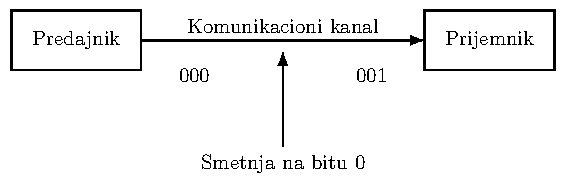
\includegraphics[width=0.9\linewidth]{Uvod/kanal}
\caption{Prenos kodne reči kroz kanal sa smetnjom.}\label{fig:channel}
\end{figure}

% Izvor DOCX: blok 66
Na primer, neka se koristi binarni Grejov kod i neka predajnik šalje reč $000_2$. Smetnja na bitu 0 menja primljenu reč u $001_2$. Pošto je i ona dozvoljena Grejova kodna reč, prijemnik ne može otkriti grešku samo proverom pripadnosti kodu. U nastavku određujemo osobine koje kod mora imati da bi omogućio detekciju grešaka.



% Izvor DOCX: blok 67
Za opis razlike između dve reči uvodimo \textbf{Hamingovo rastojanje (H\textsubscript{d})} koje predstavlja broj mesta na kojima se razlikuju dve binarne reči iste dužine. Na primer, ako imamo binarnu predstavu broja A koja je jednaka 0110110\textsubscript{2} i broja B koja je jednaka 0110010\textsubscript{2}, Hamingovo rastojanje je jednako 1, što zapisujemo:



% Izvor DOCX: blok 68
\begin{equation}\label{eq:1.1.3.1}
H_{d}(A,B) = d(0110110_{2},0110010_{2}) = 1
\end{equation}


% Izvor DOCX: blok 69
Skup svih $n$-bitnih reči ima $2^n$ elemenata. Predstavlja se temenima $n$-dimenzione kocke, pri čemu su ivicom spojene reči Hamingovog rastojanja 1. Primeri za $n=1,2,3$ dati su na slici~\ref{fig:cube}.


% Izvor DOCX: blok 70
\begin{figure}[!htbp]\centering
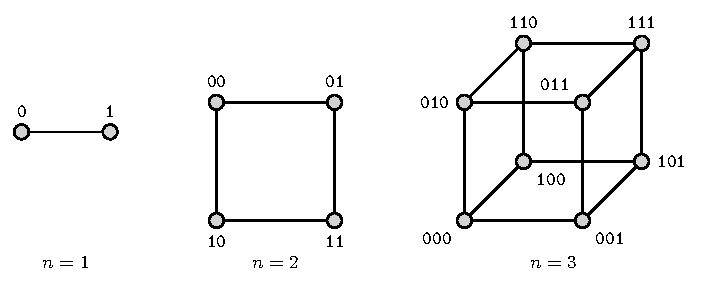
\includegraphics[width=0.9\linewidth]{Uvod/kocke}
\caption{Geometrijska interpretacija Hamingovog rastojanja.}\label{fig:cube}
\end{figure}

% Izvor DOCX: blok 71
Minimalno Hamingovo rastojanje $d_{\min}$ je najmanje rastojanje između dve \emph{različite} dozvoljene reči. Tabela~\ref{tab:distances} prikazuje primere za BCD8421.

% Izvor DOCX: blok 72


% Izvor DOCX: blok 73
\begin{table}[!htbp]\centering\caption{Primeri Hamingovih rastojanja u BCD kodu.}\label{tab:distances}
\begin{adjustbox}{max width=\linewidth}\begin{tabular}{cc}\toprule
Prva grupa & Druga grupa\\\midrule
$d(000\istaknutbit{0},000\istaknutbit{1})=1$ & $d(000\istaknutbit{1},000\istaknutbit{0})=1$\\
\redlinija
$d(00\istaknutbit{0}0,00\istaknutbit{1}0)=1$ & $d(00\istaknutbit{0}\istaknutbit{1},00\istaknutbit{1}\istaknutbit{0})=2$\\
\redlinija
$d(00\istaknutbit{0}\istaknutbit{0},00\istaknutbit{1}\istaknutbit{1})=2$ & $d(00\istaknutbit{0}1,00\istaknutbit{1}1)=1$\\
\redlinija
$d(0\istaknutbit{0}00,0\istaknutbit{1}00)=1$ & $d(0\istaknutbit{0}0\istaknutbit{1},0\istaknutbit{1}0\istaknutbit{0})=2$\\
\redlinija
$d(0\istaknutbit{0}0\istaknutbit{0},0\istaknutbit{1}0\istaknutbit{1})=2$ & $d(0\istaknutbit{0}01,0\istaknutbit{1}01)=1$\\
\redlinija
$d(0\istaknutbit{0}\istaknutbit{0}0,0\istaknutbit{1}\istaknutbit{1}0)=2$ & $\cdots$\\
\redlinija
$d(0\istaknutbit{0}\istaknutbit{0}\istaknutbit{0},0\istaknutbit{1}\istaknutbit{1}\istaknutbit{1})=3$ & \\
\redlinija
$d(\istaknutbit{0}000,\istaknutbit{1}000)=1$ & \\
\redlinija
$d(\istaknutbit{0}00\istaknutbit{0},\istaknutbit{1}00\istaknutbit{1})=2$ & \\
\bottomrule\end{tabular}\end{adjustbox}
\end{table}


% Izvor DOCX: blok 74
Kod rastojanja $d_{\min}$ garantovano detektuje svaku grešku koja menja najviše $d_{\min}-1$ bita, ako se koristi samo detekcija. Za $d_{\min}=1$ nema garancije detekcije proizvoljne jednobitne greške, iako se neke konkretne greške mogu detektovati. Za korekciju do $t$ grešaka potrebno je $d_{\min}\ge2t+1$.

% Izvor DOCX: blok 75
Za istovremenu korekciju do $n_c$ grešaka i detekciju do ukupno $n_d$ grešaka, uz $n_d\ge n_c$, dovoljan i za garanciju zasnovanu na rastojanju potreban uslov je:

% Izvor DOCX: blok 76
\begin{equation}\label{eq:1.1.3.2}
d_{\min}\ge n_c+n_d+1,\qquad n_d\ge n_c.
\end{equation}


% Izvor DOCX: blok 77
gde je



% Izvor DOCX: blok 78
\begin{itemize}[leftmargin=*]
\item $n_c$: najveći broj grešaka koje se garantovano koriguju;
\item $n_d$: najveći ukupan broj grešaka koje se garantovano detektuju u istom režimu.
\end{itemize}
Da bi reč sa najviše $n_d$ grešaka bila pogrešno korigovana u drugu reč udaljenu najviše $n_c$, dve dozvoljene reči morale bi biti udaljene najviše $n_c+n_d$, što navedeni uslov isključuje.

% Izvor DOCX: blok 79
\Needspace{6\baselineskip}
\textbf{Kod sa parnom i neparnom parnošću}



% Izvor DOCX: blok 80
Kod parne parnosti ukupan broj jedinica je paran, a kod neparne neparan. U ovim primerima bit parnosti dodaje se zdesna. Za parnu parnost $p=d_{m-1}\oplus\dots\oplus d_0$, a za neparnu koristi se $\bar p$. Tabela~\ref{tab:parity3} prikazuje sve trobitne poruke.


% Izvor DOCX: blok 81
\begin{table}[!htbp]\centering\caption{Kodiranje trobitnih poruka bitom parnosti.}\label{tab:parity3}
\begin{adjustbox}{max width=\linewidth}\begin{tabular}{ccc}\toprule
Informacioni biti & Parna parnost & Neparna parnost\\\midrule
000 & 000\istaknutbit{0} & 000\istaknutbit{1}\\
\redlinija
001 & 001\istaknutbit{1} & 001\istaknutbit{0}\\
\redlinija
010 & 010\istaknutbit{1} & 010\istaknutbit{0}\\
\redlinija
011 & 011\istaknutbit{0} & 011\istaknutbit{1}\\
\redlinija
100 & 100\istaknutbit{1} & 100\istaknutbit{0}\\
\redlinija
101 & 101\istaknutbit{0} & 101\istaknutbit{1}\\
\redlinija
110 & 110\istaknutbit{0} & 110\istaknutbit{1}\\
\redlinija
111 & 111\istaknutbit{1} & 111\istaknutbit{0}\\
\bottomrule\end{tabular}\end{adjustbox}
\end{table}


% Izvor DOCX: blok 82


% Izvor DOCX: blok 83
Za fiksnu dužinu poruke oba koda imaju $d_{\min}=2$. Otkrivaju svaku grešku sa neparnim brojem promenjenih bita, ali ne i greške sa parnim brojem. Sam bit parnosti ne određuje položaj greške i ne omogućava njenu korekciju.

% Izvor DOCX: blok 84
\Needspace{6\baselineskip}
\textbf{Hamingov kod}



% Izvor DOCX: blok 85
Osnovni Hamingov kod ima $d_{\min}=3$: koriguje jednu grešku, ili detektuje do dve greške kada se koristi samo detekcija. Sam sindrom ne razlikuje svaku dvobitnu grešku od jednobitne. Za istovremenu korekciju jedne i detekciju dve greške dodaje se opšti bit parnosti, čime se dobija prošireni kod sa $d_{\min}=4$. Za osnovni Hamingov kod (pre dodavanja opšteg bita parnosti), broj kontrolnih bita $r$ za $m$ informacionih bita mora zadovoljiti:

% Izvor DOCX: blok 86
\begin{equation}\label{eq:1.1.3.3}
2^{r} \geq m + r + 1
\end{equation}


% Izvor DOCX: blok 87
dok je dužina kodne reči definisana sa:



% Izvor DOCX: blok 88
\begin{equation}\label{eq:1.1.3.4}
n=m+r\le2^r-1
\end{equation}


% Izvor DOCX: blok 89
Na osnovu \eqref{eq:1.1.3.3} dobijamo da je maksimalan broj informacionih bita \emph{m} koje je moguće zaštititi sa \emph{r} kontrolnih bita definisan relacijom:



% Izvor DOCX: blok 90
\begin{equation}\label{eq:1.1.3.5}
m_{\max}=2^r-r-1
\end{equation}


% Izvor DOCX: blok 91
Kodna reč se formira na sledeći način:



% Izvor DOCX: blok 92
\begin{enumerate}[label=\arabic*.,start=1,leftmargin=*]
\item Pozicije bita u kodnoj reči numerišu se zdesna nalevo, počev od 1, i zapisuju se binarno.

\end{enumerate}


% Izvor DOCX: blok 93
\begin{center}\begin{minipage}{\linewidth}\centering\captionsetup{hypcap=false}
\captionof{table}{Numeracija pozicija u petnaestobitnoj reči.}\label{tab:pozicije}
\begin{adjustbox}{max width=\linewidth}
\begin{tabular}{ccccccccccccccc}\toprule
15 & 14 & 13 & 12 & 11 & 10 & 9 & 8 & 7 & 6 & 5 & 4 & 3 & 2 & 1 \\
\midrule
1111 & 1110 & 1101 & 1100 & 1011 & 1010 & 1001 & 1000 & 0111 & 0110 & 0101 & 0100 & 0011 & 0010 & 0001 \\
\bottomrule\end{tabular}\end{adjustbox}\end{minipage}\end{center}


% Izvor DOCX: blok 94
\begin{enumerate}[label=\arabic*.,start=2,leftmargin=*]
\item Kontrolni biti se u okviru kodne reči postavljaju na pozicijama koje odgovaraju stepenu broja 2 (1, 2, 4, 8, \ldots{})

\end{enumerate}


% Izvor DOCX: blok 95
\begin{center}\begin{minipage}{\linewidth}\centering\captionsetup{hypcap=false}
\captionof{table}{Kontrolni biti na pozicijama koje su stepeni broja 2.}\label{tab:kontrolni}
\begin{adjustbox}{max width=\linewidth}
\begin{tabular}{ccccccccccccccc}\toprule
15 & 14 & 13 & 12 & 11 & 10 & 9 & 8 & 7 & 6 & 5 & 4 & 3 & 2 & 1 \\
\midrule
1111 & 1110 & 1101 & 1100 & 1011 & 1010 & 1001 & 1000 & 0111 & 0110 & 0101 & 0100 & 0011 & 0010 & 0001 \\
\redlinija
 &  &  &  &  &  &  & C\textsubscript{8} &  &  &  & C\textsubscript{4} &  & C\textsubscript{2} & C\textsubscript{1} \\
\bottomrule\end{tabular}\end{adjustbox}\end{minipage}\end{center}


% Izvor DOCX: blok 96
\begin{enumerate}[label=\arabic*.,start=3,leftmargin=*]
\item Informacioni biti se postavljaju na preostala mesta u kodnoj reči

\end{enumerate}


% Izvor DOCX: blok 97
\begin{center}\begin{minipage}{\linewidth}\centering\captionsetup{hypcap=false}
\captionof{table}{Raspored kontrolnih i informacionih bita.}\label{tab:informacioni}
\begin{adjustbox}{max width=\linewidth}
\begin{tabular}{ccccccccccccccc}\toprule
15 & 14 & 13 & 12 & 11 & 10 & 9 & 8 & 7 & 6 & 5 & 4 & 3 & 2 & 1 \\
\midrule
1111 & 1110 & 1101 & 1100 & 1011 & 1010 & 1001 & 1000 & 0111 & 0110 & 0101 & 0100 & 0011 & 0010 & 0001 \\
\redlinija
D\textsubscript{10} & D\textsubscript{9} & D\textsubscript{8} & D\textsubscript{7} & D\textsubscript{6} & D\textsubscript{5} & D\textsubscript{4} & C\textsubscript{8} & D\textsubscript{3} & D\textsubscript{2} & D\textsubscript{1} & C\textsubscript{4} & D\textsubscript{0} & C\textsubscript{2} & C\textsubscript{1} \\
\bottomrule\end{tabular}\end{adjustbox}\end{minipage}\end{center}


% Izvor DOCX: blok 98
\begin{enumerate}[label=\arabic*.,start=4,leftmargin=*]
\item Kontrolni bit na poziciji $i=2^k$ pripada grupi svih pozicija čiji binarni indeks ima jedinicu na mestu $k$. Pri kodovanju bira se tako da cela grupa, uključujući njega, ima zadatu parnost. Pri proveri se računa parnost cele grupe; kontrolni bit se ne izračunava XOR-om grupe koja već uključuje njega samog.

\end{enumerate}


% Izvor DOCX: blok 99
\begin{center}\begin{minipage}{\linewidth}\centering\captionsetup{hypcap=false}
\captionof{table}{Raspored bita za formiranje kontrolnih grupa.}\label{tab:raspored-provera}
\begingroup\small\setlength{\tabcolsep}{3pt}
\begin{tabular}{ccccccccccccccc}\toprule
15 & 14 & 13 & 12 & 11 & 10 & 9 & 8 & 7 & 6 & 5 & 4 & 3 & 2 & 1 \\
\midrule
1111 & 1110 & 1101 & 1100 & 1011 & 1010 & 1001 & 1000 & 0111 & 0110 & 0101 & 0100 & 0011 & 0010 & 0001 \\
\redlinija
\tikzmarknode[inner sep=0pt]{hamming-15}{\strut D\textsubscript{10}} & \tikzmarknode[inner sep=0pt]{hamming-14}{\strut D\textsubscript{9}} & \tikzmarknode[inner sep=0pt]{hamming-13}{\strut D\textsubscript{8}} & \tikzmarknode[inner sep=0pt]{hamming-12}{\strut D\textsubscript{7}} & \tikzmarknode[inner sep=0pt]{hamming-11}{\strut D\textsubscript{6}} & \tikzmarknode[inner sep=0pt]{hamming-10}{\strut D\textsubscript{5}} & \tikzmarknode[inner sep=0pt]{hamming-9}{\strut D\textsubscript{4}} & \cellcolor{violet!12}\tikzmarknode[inner sep=0pt]{hamming-8}{\strut C\textsubscript{8}} & \tikzmarknode[inner sep=0pt]{hamming-7}{\strut D\textsubscript{3}} & \tikzmarknode[inner sep=0pt]{hamming-6}{\strut D\textsubscript{2}} & \tikzmarknode[inner sep=0pt]{hamming-5}{\strut D\textsubscript{1}} & \cellcolor{orange!16}\tikzmarknode[inner sep=0pt]{hamming-4}{\strut C\textsubscript{4}} & \tikzmarknode[inner sep=0pt]{hamming-3}{\strut D\textsubscript{0}} & \cellcolor{teal!12}\tikzmarknode[inner sep=0pt]{hamming-2}{\strut C\textsubscript{2}} & \cellcolor{Primary!15}\tikzmarknode[inner sep=0pt]{hamming-1}{\strut C\textsubscript{1}} \\
\bottomrule\end{tabular}
\begin{tikzpicture}[remember picture,overlay,line width=.55pt,>={Latex[length=1.4mm,width=1mm]}]
% The source control bit belongs to its group; arrows show the other positions.
\foreach \control/\level/\offset/\groupcolor/\targets in {
  1/.35/.15/Primary/{3,5,7,9,11,13,15},
  2/.70/.05/teal!75!black/{3,6,7,10,11,14,15},
  4/1.05/-.05/orange!85!black/{5,6,7,12,13,14,15},
  8/1.40/-.15/violet!75!black/{9,10,11,12,13,14,15}}
{
  \coordinate (group-start) at ([yshift=-5pt]hamming-\control.south);
  \coordinate (group-bus) at ([yshift=-\level cm]group-start);
  \coordinate (group-end) at ([xshift=\offset cm]hamming-15.south);
  \draw[\groupcolor] (group-start)--(group-bus)--(group-end |- group-bus);
  \foreach \position in \targets {
    \coordinate (group-target) at ([xshift=\offset cm,yshift=-5pt]hamming-\position.south);
    \draw[\groupcolor,->] (group-target |- group-bus)--(group-target);
  }
}
\end{tikzpicture}
\par\vspace{1.65cm}\endgroup
\end{minipage}\end{center}

\begin{center}\begin{minipage}{\linewidth}\centering\captionsetup{hypcap=false}
\captionof{table}{Pozicije uključene u svaku proveru parnosti.}\label{tab:grupe}

\begin{adjustbox}{max width=\linewidth}\begin{tabular}{cc}\toprule
Kontrolni bit & Pozicije koje učestvuju u proveri\\\midrule
$c_1$ & 1, 3, 5, 7, 9, 11, 13, 15\\
\redlinija
$c_2$ & 2, 3, 6, 7, 10, 11, 14, 15\\
\redlinija
$c_4$ & 4, 5, 6, 7, 12, 13, 14, 15\\
\redlinija
$c_8$ & 8, 9, 10, 11, 12, 13, 14, 15\\
\bottomrule\end{tabular}\end{adjustbox}
\end{minipage}\end{center}

% Izvor DOCX: blok 100
Za Hamingov kod dužine 7, Venov dijagram na slici~\ref{fig:venn} prikazuje koje kontrolne grupe sadrže pojedine pozicije. Oznake $d_3,d_5,d_6,d_7$ ovde sadrže \emph{pozicije u reči}, dok $D_0,\dots,D_{10}$ u prethodnim tabelama označavaju redne brojeve informacionih bita.

% Izvor DOCX: blok 101
\begin{figure}[!htbp]\centering
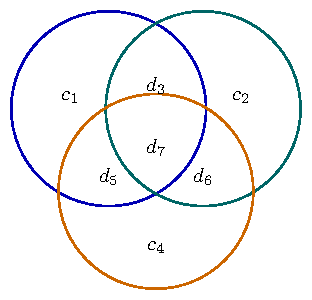
\includegraphics[width=0.52\linewidth]{Uvod/ven}
\caption{Kontrolne grupe Hamingovog koda (7,4).}\label{fig:venn}
\end{figure}

% Izvor DOCX: blok 102
Sindrom se dobija ponovnim izračunavanjem parnosti svake kontrolne grupe: $s_j=0$ ako provera prolazi, a $s_j=1$ ako ne prolazi. Za najviše jednu grešku broj $(s_4s_2s_1)_2$ daje njenu poziciju. Nulti sindrom znači da su provere zadovoljene; bez ograničenja broja grešaka to nije dokaz da greške nema.

% Izvor DOCX: blok 103
\FloatBarrier
\clearpage
\section{Zadaci sa časova vežbi}\label{sec:2}


% Izvor DOCX: blok 104
\FloatBarrier
\subsection{Zadatak 1}\label{sec:2.1}


% Izvor DOCX: blok 105
\begin{enumerate}[label=\alph*),start=1,leftmargin=*]
\item Predstaviti sledeće decimalne brojeve u BCD kodu, kodu više 3, Grejovom BCD kodu, BCD2421 kodu i Grejovom binarnom kodu:

\end{enumerate}


% Izvor DOCX: blok 106
43, 0, 15, 49, 62



% Izvor DOCX: blok 107
Navesti težine bita za težinske kodove i obrazložiti zašto ostali navedeni kodovi nemaju takve fiksne težine.

% Izvor DOCX: blok 108
\begin{enumerate}[label=\alph*),start=2,leftmargin=*]
\item Sledeće binarne brojeve prebaciti u decimalni brojni sistem ukoliko se interpretiraju kao brojevi zapisani u BCD kodu, kodu više 3, Grejovom BCD kodu, BCD2421 kodu i Grejovom binarnom kodu:

\end{enumerate}


% Izvor DOCX: blok 109
101001.100101, 10010011.1110101, 1011.101001

\napomena{Za kodove decimalnih cifara usvajamo da su izostavljene samo spoljne nule: nepotpunu četvorku celog dela dopunjujemo sleva, a razlomljenog dela zdesna. To je pretpostavka o datim nizovima, a ne opšte pravilo očuvanja vrednosti pri produžavanju kodnih reči. Za binarni Grejov kod primenjujemo Grejovo kodovanje celog niza bita kao neoznačenog skaliranog celog broja; po dekodiranju zadržavamo izvorni broj razlomljenih bita.}



% Izvor DOCX: blok 110
\subsubsection*{Rešenje:}


% Izvor DOCX: blok 111
\begin{enumerate}[label=\alph*),start=1,leftmargin=*]
\item Na osnovu postupka opisanog u odeljku~\ref{sec:1.1} dobijamo:

\end{enumerate}


% Izvor DOCX: blok 112
\begin{center}\begin{minipage}{\linewidth}\centering\captionsetup{hypcap=false}
\captionof{table}{Kodovanje zadatih decimalnih brojeva.}\label{tab:kodiranje}

\begin{adjustbox}{max width=\linewidth}\begin{tabular}{ccccc>{\centering\arraybackslash}p{4.3cm}}\toprule
Broj & BCD & BCD2421 & Više 3 & Grej BCD & Grej binarni\\\midrule
43 & 0100 0011 & 0100 0011 & 0111 0110 & 0110 0010 & $101011_2\;\to\;111110_{\mathrm{G}}$\\
\redlinija
0 & 0000 & 0000 & 0011 & 0000 & $000000_2\;\to\;000000_{\mathrm{G}}$\\
\redlinija
15 & 0001 0101 & 0001 1011 & 0100 1000 & 0001 0111 & $001111_2\;\to\;001000_{\mathrm{G}}$\\
\redlinija
49 & 0100 1001 & 0100 1111 & 0111 1100 & 0110 1000 & $110001_2\;\to\;101001_{\mathrm{G}}$\\
\redlinija
62 & 0110 0010 & 1100 0010 & 1001 0101 & 0101 0011 & $111110_2\;\to\;100001_{\mathrm{G}}$\\
\bottomrule\end{tabular}\end{adjustbox}
\end{minipage}\end{center}

Za BCD8421 težine su $(8,4,2,1)$, a za BCD2421 $(2,4,2,1)$. Kod „više 3“ i oba ovde korišćena Grejova koda nemaju fiksne aditivne težine. Za „više 3“, reči za cifre $0,1,2,3$ zahtevale bi redom $w_1+w_0=0$, $w_2=1$, $w_2+w_0=2$, $w_2+w_1=3$. Poslednje tri daju $w_0=1$, $w_1=2$, suprotno prvom uslovu. Za oba Grejova koda početne reči $00,01,11,10$ za brojeve $0,1,2,3$ zahtevale bi $w_0=1$, $w_1+w_0=2$ i $w_1=3$, što je takođe protivrečno. Vodeće nule ne utiču na ovaj dokaz. Binarni Grejov kod ovde ima šest bita, dovoljno za sve zadate brojeve. U poslednjoj koloni prikazani su početni binarni zapis (indeks 2) i dobijena Grejova kodna reč (oznaka G).\par

% Izvor DOCX: blok 113
Primenom pretpostavki iz postavke dobijamo tabelu~\ref{tab:dekodiranje}. Svaka četvorka decimalnog koda mora biti dozvoljena; znak „--“ označava nedozvoljenu reč. Kod binarnog Grejovog zapisa tačka se vraća tek posle dekodiranja celog niza, bez dopisivanja bita.

% Izvor DOCX: blok 114
\begin{center}\begin{minipage}{\linewidth}\centering\captionsetup{hypcap=false}
\captionof{table}{Dekodiranje zadatih nizova uz usvojene pretpostavke.}\label{tab:dekodiranje}

\begingroup\setlength{\tabcolsep}{4pt}
\begin{adjustbox}{max width=\linewidth}\begin{tabular}{ccccc>{\centering\arraybackslash}p{6.3cm}}\toprule
Izvorna reč & BCD & BCD2421 & Više 3 & Grej BCD & Grej binarni\\\midrule
101001.100101 & 29.94 & -- & -- & -- & $110001.000110_2=49.09375_{10}$\\
\redlinija
10010011.1110101 & -- & -- & -- & -- & $11100010.1011001_2=226.6953125_{10}$\\
\redlinija
1011.101001 & -- & -- & 8.71 & -- & $1101.001110_2=13.21875_{10}$\\
\bottomrule\end{tabular}\end{adjustbox}\endgroup
\end{minipage}\end{center}


% Izvor DOCX: blok 115


% Izvor DOCX: blok 116
\FloatBarrier
\subsection{Zadatak 2}\label{sec:2.2}


% Izvor DOCX: blok 117
Izvršiti sledeća sabiranja decimalnih brojeva u BCD kodu:



% Izvor DOCX: blok 118
34 + 13, 35 + 86, 1026 + 192, 529 + 432



% Izvor DOCX: blok 119
\subsubsection*{Rešenje:}


% Izvor DOCX: blok 120
Sabiraju se po dve BCD cifre sa ulaznim decimalnim prenosom. Ako puni binarni zbir prelazi 9, tj. ako je četvorobitni rezultat veći od 1001 \emph{ili} postoji izlazni binarni prenos, dodaje se korekcija 0110. Zatim se cifra i decimalni prenos prosleđuju u sledeći korak. Postupak ide zdesna nalevo, od pozicije $i=0$. U međurezultatima se već dobijene niže BCD cifre prepisuju; plavom bojom istaknuti su ulazni prenos i korekcija.

% Izvor DOCX: blok 121
\begin{center}\begin{minipage}{\linewidth}\centering\captionsetup{hypcap=false}
\captionof{table}{BCD sabiranje $34+13$ — pisani postupak.}\label{tab:zbir-1}
\begingroup\small\setlength{\arraycolsep}{2pt}\renewcommand{\arraystretch}{1.12}
\begin{adjustbox}{max width=\linewidth}\begin{tabular}{@{}c@{}}\toprule
$\begin{array}{r*{9}{c}@{}c@{}l}
\multicolumn{10}{c}{\text{Pisani postupak}} & \rule{8mm}{0pt} & \text{Objašnjenje}\\\midrule
% BCD korak 0
 &  & 0 & 0 & 1 & 1 & 0 & 1 & 0 & 0 & & i=0:\ \text{prvi sabirak} \\
+ &  & 0 & 0 & 0 & 1 & 0 & 0 & 1 & 1 & & \text{Drugi sabirak} \\
\cline{6-10}
 &  &  &  &  & 0 & 0 & 1 & 1 & 1 & & \text{Nema korekcije; }c_1=0 \\
\noalign{\vskip 5pt}
% BCD korak 1
 &  & 0 & 0 & 1 & 1 &  &  &  &  & & i=1:\ \text{prvi sabirak} \\
+ &  & 0 & 0 & 0 & 1 &  &  &  &  & & \text{Drugi sabirak} \\
\cline{2-10}
 & 0 & 0 & 1 & 0 & 0 & 0 & 1 & 1 & 1 & & \text{Nema korekcije; }c_2=0 \\
\end{array}$\\\bottomrule\end{tabular}
\end{adjustbox}\endgroup
\begin{equation}\label{eq:bcd-zbir-1}
34+13=47\quad\longleftrightarrow\quad \mathtt{0100\,0111}
\end{equation}
\end{minipage}\end{center}

\begin{center}\begin{minipage}{\linewidth}\centering\captionsetup{hypcap=false}
\captionof{table}{BCD sabiranje $35+86$ — pisani postupak.}\label{tab:zbir-2}
\begingroup\small\setlength{\arraycolsep}{2pt}\renewcommand{\arraystretch}{1.12}
\begin{adjustbox}{max width=\linewidth}\begin{tabular}{@{}c@{}}\toprule
$\begin{array}{r*{9}{c}@{}c@{}l}
\multicolumn{10}{c}{\text{Pisani postupak}} & \rule{8mm}{0pt} & \text{Objašnjenje}\\\midrule
% BCD korak 0
 &  & 0 & 0 & 1 & 1 & 0 & 1 & 0 & 1 & & i=0:\ \text{prvi sabirak} \\
+ &  & 1 & 0 & 0 & 0 & 0 & 1 & 1 & 0 & & \text{Drugi sabirak} \\
\cline{6-10}
 &  &  &  &  & 0 & 1 & 0 & 1 & 1 & & \text{Binarni zbir; potrebna korekcija} \\
+ &  &  &  &  &  & \istaknutbit{0} & \istaknutbit{1} & \istaknutbit{1} & \istaknutbit{0} & & \text{Korekcija }0110_2 \\
\cline{6-10}
 &  &  &  &  & 1 & 0 & 0 & 0 & 1 & & \text{Korigovana cifra; }c_1=1 \\
\noalign{\vskip 5pt}
% BCD korak 1
 &  & 0 & 0 & 1 & 1 &  &  &  &  & & i=1:\ \text{prvi sabirak} \\
+ &  & 1 & 0 & 0 & 0 &  &  &  &  & & \text{Drugi sabirak} \\
+ &  &  &  &  & \istaknutbit{1} &  &  &  &  & & \text{Ulazni prenos }c_1=1 \\
\cline{2-10}
 & 0 & 1 & 1 & 0 & 0 & 0 & 0 & 0 & 1 & & \text{Binarni zbir; potrebna korekcija} \\
+ &  & \istaknutbit{0} & \istaknutbit{1} & \istaknutbit{1} & \istaknutbit{0} &  &  &  &  & & \text{Korekcija }0110_2 \\
\cline{2-10}
 & 1 & 0 & 0 & 1 & 0 & 0 & 0 & 0 & 1 & & \text{Korigovana cifra; }c_2=1 \\
\end{array}$\\\bottomrule\end{tabular}
\end{adjustbox}\endgroup
\begin{equation}\label{eq:bcd-zbir-2}
35+86=121\quad\longleftrightarrow\quad \mathtt{0001\,0010\,0001}
\end{equation}
\end{minipage}\end{center}

\begin{center}\begin{minipage}{\linewidth}\centering\captionsetup{hypcap=false}
\captionof{table}{BCD sabiranje $1026+192$ — pisani postupak.}\label{tab:zbir-3}
\begingroup\small\setlength{\arraycolsep}{2pt}\renewcommand{\arraystretch}{1.12}
\begin{adjustbox}{max width=\linewidth}\begin{tabular}{@{}c@{}}\toprule
$\begin{array}{r*{17}{c}@{}c@{}l}
\multicolumn{18}{c}{\text{Pisani postupak}} & \rule{8mm}{0pt} & \text{Objašnjenje}\\\midrule
% BCD korak 0
 &  & 0 & 0 & 0 & 1 & 0 & 0 & 0 & 0 & 0 & 0 & 1 & 0 & 0 & 1 & 1 & 0 & & i=0:\ \text{prvi sabirak} \\
+ &  & 0 & 0 & 0 & 0 & 0 & 0 & 0 & 1 & 1 & 0 & 0 & 1 & 0 & 0 & 1 & 0 & & \text{Drugi sabirak} \\
\cline{14-18}
 &  &  &  &  &  &  &  &  &  &  &  &  & 0 & 1 & 0 & 0 & 0 & & \text{Nema korekcije; }c_1=0 \\
\noalign{\vskip 5pt}
% BCD korak 1
 &  &  &  &  &  &  &  &  &  & 0 & 0 & 1 & 0 &  &  &  &  & & i=1:\ \text{prvi sabirak} \\
+ &  &  &  &  &  &  &  &  &  & 1 & 0 & 0 & 1 &  &  &  &  & & \text{Drugi sabirak} \\
\cline{10-18}
 &  &  &  &  &  &  &  &  & 0 & 1 & 0 & 1 & 1 & 1 & 0 & 0 & 0 & & \text{Binarni zbir; potrebna korekcija} \\
+ &  &  &  &  &  &  &  &  &  & \istaknutbit{0} & \istaknutbit{1} & \istaknutbit{1} & \istaknutbit{0} &  &  &  &  & & \text{Korekcija }0110_2 \\
\cline{10-18}
 &  &  &  &  &  &  &  &  & 1 & 0 & 0 & 0 & 1 & 1 & 0 & 0 & 0 & & \text{Korigovana cifra; }c_2=1 \\
\noalign{\vskip 5pt}
% BCD korak 2
 &  &  &  &  &  & 0 & 0 & 0 & 0 &  &  &  &  &  &  &  &  & & i=2:\ \text{prvi sabirak} \\
+ &  &  &  &  &  & 0 & 0 & 0 & 1 &  &  &  &  &  &  &  &  & & \text{Drugi sabirak} \\
+ &  &  &  &  &  &  &  &  & \istaknutbit{1} &  &  &  &  &  &  &  &  & & \text{Ulazni prenos }c_2=1 \\
\cline{6-18}
 &  &  &  &  & 0 & 0 & 0 & 1 & 0 & 0 & 0 & 0 & 1 & 1 & 0 & 0 & 0 & & \text{Nema korekcije; }c_3=0 \\
\noalign{\vskip 5pt}
% BCD korak 3
 &  & 0 & 0 & 0 & 1 &  &  &  &  &  &  &  &  &  &  &  &  & & i=3:\ \text{prvi sabirak} \\
+ &  & 0 & 0 & 0 & 0 &  &  &  &  &  &  &  &  &  &  &  &  & & \text{Drugi sabirak} \\
\cline{2-18}
 & 0 & 0 & 0 & 0 & 1 & 0 & 0 & 1 & 0 & 0 & 0 & 0 & 1 & 1 & 0 & 0 & 0 & & \text{Nema korekcije; }c_4=0 \\
\end{array}$\\\bottomrule\end{tabular}
\end{adjustbox}\endgroup
\begin{equation}\label{eq:bcd-zbir-3}
1026+192=1218\quad\longleftrightarrow\quad \mathtt{0001\,0010\,0001\,1000}
\end{equation}
\end{minipage}\end{center}

\begin{center}\begin{minipage}{\linewidth}\centering\captionsetup{hypcap=false}
\captionof{table}{BCD sabiranje $529+432$ — pisani postupak.}\label{tab:zbir-4}
\begingroup\small\setlength{\arraycolsep}{2pt}\renewcommand{\arraystretch}{1.12}
\begin{adjustbox}{max width=\linewidth}\begin{tabular}{@{}c@{}}\toprule
$\begin{array}{r*{13}{c}@{}c@{}l}
\multicolumn{14}{c}{\text{Pisani postupak}} & \rule{8mm}{0pt} & \text{Objašnjenje}\\\midrule
% BCD korak 0
 &  & 0 & 1 & 0 & 1 & 0 & 0 & 1 & 0 & 1 & 0 & 0 & 1 & & i=0:\ \text{prvi sabirak} \\
+ &  & 0 & 1 & 0 & 0 & 0 & 0 & 1 & 1 & 0 & 0 & 1 & 0 & & \text{Drugi sabirak} \\
\cline{10-14}
 &  &  &  &  &  &  &  &  & 0 & 1 & 0 & 1 & 1 & & \text{Binarni zbir; potrebna korekcija} \\
+ &  &  &  &  &  &  &  &  &  & \istaknutbit{0} & \istaknutbit{1} & \istaknutbit{1} & \istaknutbit{0} & & \text{Korekcija }0110_2 \\
\cline{10-14}
 &  &  &  &  &  &  &  &  & 1 & 0 & 0 & 0 & 1 & & \text{Korigovana cifra; }c_1=1 \\
\noalign{\vskip 5pt}
% BCD korak 1
 &  &  &  &  &  & 0 & 0 & 1 & 0 &  &  &  &  & & i=1:\ \text{prvi sabirak} \\
+ &  &  &  &  &  & 0 & 0 & 1 & 1 &  &  &  &  & & \text{Drugi sabirak} \\
+ &  &  &  &  &  &  &  &  & \istaknutbit{1} &  &  &  &  & & \text{Ulazni prenos }c_1=1 \\
\cline{6-14}
 &  &  &  &  & 0 & 0 & 1 & 1 & 0 & 0 & 0 & 0 & 1 & & \text{Nema korekcije; }c_2=0 \\
\noalign{\vskip 5pt}
% BCD korak 2
 &  & 0 & 1 & 0 & 1 &  &  &  &  &  &  &  &  & & i=2:\ \text{prvi sabirak} \\
+ &  & 0 & 1 & 0 & 0 &  &  &  &  &  &  &  &  & & \text{Drugi sabirak} \\
\cline{2-14}
 & 0 & 1 & 0 & 0 & 1 & 0 & 1 & 1 & 0 & 0 & 0 & 0 & 1 & & \text{Nema korekcije; }c_3=0 \\
\end{array}$\\\bottomrule\end{tabular}
\end{adjustbox}\endgroup
\begin{equation}\label{eq:bcd-zbir-4}
529+432=961\quad\longleftrightarrow\quad \mathtt{1001\,0110\,0001}
\end{equation}
\end{minipage}\end{center}


% Izvor DOCX: blok 122
\FloatBarrier
\subsection{Zadatak 3}\label{sec:2.3}


% Izvor DOCX: blok 123
\begin{enumerate}[label=\alph*),start=1,leftmargin=*]
\item Odrediti Hamingovo rastojanje sledećih kodnih reči:

\end{enumerate}


% Izvor DOCX: blok 124
100 i 101, 110 i 011, 011 i 100



% Izvor DOCX: blok 125
\begin{enumerate}[label=\alph*),start=2,leftmargin=*]
\item Za dekadni broj 23, odrediti sve brojeve koji su na Hamingovom rastojanju 1 od njega, ukoliko je broj predstavljen u BCD kodu, kodu više 3, Grejovom BCD kodu, BCD 2421 kodu i Grejovom binarnom kodu.

\end{enumerate}


% Izvor DOCX: blok 126
\Needspace{10\baselineskip}
\subsubsection*{Rešenje:}


% Izvor DOCX: blok 127
\begin{enumerate}[label=\alph*),start=1,leftmargin=*]
\item Na osnovu definicije Hamingovog rastojanja predstavljene u odeljku~\ref{sec:1.1.3} važi:

\end{enumerate}


% Izvor DOCX: blok 128
10\istaknutbit{0} : 10\istaknutbit{1} \ensuremath{\to} H\textsubscript{d} = 1

% Izvor DOCX: blok 129
\istaknutbit{1}1\istaknutbit{0} : \istaknutbit{0}1\istaknutbit{1} \ensuremath{\to} H\textsubscript{d} = 2

% Izvor DOCX: blok 130
\istaknutbit{0}\istaknutbit{1}\istaknutbit{1} : \istaknutbit{1}\istaknutbit{0}\istaknutbit{0} \ensuremath{\to} H\textsubscript{d} = 3

% Izvor DOCX: blok 131
\begin{enumerate}[label=\alph*),start=2,leftmargin=*]
\item Na osnovu odeljka~\ref{sec:1.1.3} važi:

\end{enumerate}

% Izvor DOCX: blok 132
Za kodove decimalnih cifara koristimo osam bita, a za binarni Grejov kod pet bita. Skup suseda zavisi od te širine; vodeće nule u većoj širini dale bi dodatne susede. Biti su numerisani zdesna nalevo, počev od 0; plavom bojom označen je promenjeni bit. Svaki red prikazuje jednu promenu početne reči, a zatim njeno dekodovanje.\par

\par\noindent\begin{minipage}{\linewidth}
\textbf{BCD}: $23\leftrightarrow\mathtt{0010\,0011}$.\par
\begin{center}\centering\captionsetup{hypcap=false}
\captionof{table}{Jednobitni susedi broja 23 u kodu BCD8421.}\label{tab:susedi-bcd}
\begin{adjustbox}{max width=\linewidth}\begin{tabular}{ccc}\toprule
Promenjen bit & Promenjena reč & Dekodovanje\\\midrule
7 & $\mathtt{\istaknutbit{1}010\,0011}$ & Nedozvoljena reč: $\mathtt{1010}$ nije kod cifre\\
\redlinija
6 & $\mathtt{0\istaknutbit{1}10\,0011}$ & $\mathtt{0110}\to6,\;\mathtt{0011}\to3\;\Rightarrow 63$\\
\redlinija
5 & $\mathtt{00\istaknutbit{0}0\,0011}$ & $\mathtt{0000}\to0,\;\mathtt{0011}\to3\;\Rightarrow 03$\\
\redlinija
4 & $\mathtt{001\istaknutbit{1}\,0011}$ & $\mathtt{0011}\to3,\;\mathtt{0011}\to3\;\Rightarrow 33$\\
\redlinija
3 & $\mathtt{0010\,\istaknutbit{1}011}$ & Nedozvoljena reč: $\mathtt{1011}$ nije kod cifre\\
\redlinija
2 & $\mathtt{0010\,0\istaknutbit{1}11}$ & $\mathtt{0010}\to2,\;\mathtt{0111}\to7\;\Rightarrow 27$\\
\redlinija
1 & $\mathtt{0010\,00\istaknutbit{0}1}$ & $\mathtt{0010}\to2,\;\mathtt{0001}\to1\;\Rightarrow 21$\\
\redlinija
0 & $\mathtt{0010\,001\istaknutbit{0}}$ & $\mathtt{0010}\to2,\;\mathtt{0010}\to2\;\Rightarrow 22$\\
\bottomrule\end{tabular}\end{adjustbox}
\end{center}
\end{minipage}\par\medskip

\par\noindent\begin{minipage}{\linewidth}
\textbf{BCD2421}: $23\leftrightarrow\mathtt{0010\,0011}$.\par
\begin{center}\centering\captionsetup{hypcap=false}
\captionof{table}{Jednobitni susedi broja 23 u kodu BCD2421.}\label{tab:susedi-2421}
\begin{adjustbox}{max width=\linewidth}\begin{tabular}{ccc}\toprule
Promenjen bit & Promenjena reč & Dekodovanje\\\midrule
7 & $\mathtt{\istaknutbit{1}010\,0011}$ & Nedozvoljena reč: $\mathtt{1010}$ nije kod cifre\\
\redlinija
6 & $\mathtt{0\istaknutbit{1}10\,0011}$ & Nedozvoljena reč: $\mathtt{0110}$ nije kod cifre\\
\redlinija
5 & $\mathtt{00\istaknutbit{0}0\,0011}$ & $\mathtt{0000}\to0,\;\mathtt{0011}\to3\;\Rightarrow 03$\\
\redlinija
4 & $\mathtt{001\istaknutbit{1}\,0011}$ & $\mathtt{0011}\to3,\;\mathtt{0011}\to3\;\Rightarrow 33$\\
\redlinija
3 & $\mathtt{0010\,\istaknutbit{1}011}$ & $\mathtt{0010}\to2,\;\mathtt{1011}\to5\;\Rightarrow 25$\\
\redlinija
2 & $\mathtt{0010\,0\istaknutbit{1}11}$ & Nedozvoljena reč: $\mathtt{0111}$ nije kod cifre\\
\redlinija
1 & $\mathtt{0010\,00\istaknutbit{0}1}$ & $\mathtt{0010}\to2,\;\mathtt{0001}\to1\;\Rightarrow 21$\\
\redlinija
0 & $\mathtt{0010\,001\istaknutbit{0}}$ & $\mathtt{0010}\to2,\;\mathtt{0010}\to2\;\Rightarrow 22$\\
\bottomrule\end{tabular}\end{adjustbox}
\end{center}
\end{minipage}\par\medskip

\par\noindent\begin{minipage}{\linewidth}
\textbf{Više 3}: $23\leftrightarrow\mathtt{0101\,0110}$.\par
\begin{center}\centering\captionsetup{hypcap=false}
\captionof{table}{Jednobitni susedi broja 23 u kodu „više 3“.}\label{tab:susedi-excess}
\begin{adjustbox}{max width=\linewidth}\begin{tabular}{ccc}\toprule
Promenjen bit & Promenjena reč & Dekodovanje\\\midrule
7 & $\mathtt{\istaknutbit{1}101\,0110}$ & Nedozvoljena reč: $\mathtt{1101}$ nije kod cifre\\
\redlinija
6 & $\mathtt{0\istaknutbit{0}01\,0110}$ & Nedozvoljena reč: $\mathtt{0001}$ nije kod cifre\\
\redlinija
5 & $\mathtt{01\istaknutbit{1}1\,0110}$ & $\mathtt{0111}\to4,\;\mathtt{0110}\to3\;\Rightarrow 43$\\
\redlinija
4 & $\mathtt{010\istaknutbit{0}\,0110}$ & $\mathtt{0100}\to1,\;\mathtt{0110}\to3\;\Rightarrow 13$\\
\redlinija
3 & $\mathtt{0101\,\istaknutbit{1}110}$ & Nedozvoljena reč: $\mathtt{1110}$ nije kod cifre\\
\redlinija
2 & $\mathtt{0101\,0\istaknutbit{0}10}$ & Nedozvoljena reč: $\mathtt{0010}$ nije kod cifre\\
\redlinija
1 & $\mathtt{0101\,01\istaknutbit{0}0}$ & $\mathtt{0101}\to2,\;\mathtt{0100}\to1\;\Rightarrow 21$\\
\redlinija
0 & $\mathtt{0101\,011\istaknutbit{1}}$ & $\mathtt{0101}\to2,\;\mathtt{0111}\to4\;\Rightarrow 24$\\
\bottomrule\end{tabular}\end{adjustbox}
\end{center}
\end{minipage}\par\medskip

\par\noindent\begin{minipage}{\linewidth}
\textbf{Grej BCD}: $23\leftrightarrow\mathtt{0011\,0010}$.\par
\begin{center}\centering\captionsetup{hypcap=false}
\captionof{table}{Jednobitni susedi broja 23 u decimalnom Grejovom kodu.}\label{tab:susedi-graybcd}
\begin{adjustbox}{max width=\linewidth}\begin{tabular}{ccc}\toprule
Promenjen bit & Promenjena reč & Dekodovanje\\\midrule
7 & $\mathtt{\istaknutbit{1}011\,0010}$ & Nedozvoljena reč: $\mathtt{1011}$ nije kod cifre\\
\redlinija
6 & $\mathtt{0\istaknutbit{1}11\,0010}$ & $\mathtt{0111}\to5,\;\mathtt{0010}\to3\;\Rightarrow 53$\\
\redlinija
5 & $\mathtt{00\istaknutbit{0}1\,0010}$ & $\mathtt{0001}\to1,\;\mathtt{0010}\to3\;\Rightarrow 13$\\
\redlinija
4 & $\mathtt{001\istaknutbit{0}\,0010}$ & $\mathtt{0010}\to3,\;\mathtt{0010}\to3\;\Rightarrow 33$\\
\redlinija
3 & $\mathtt{0011\,\istaknutbit{1}010}$ & Nedozvoljena reč: $\mathtt{1010}$ nije kod cifre\\
\redlinija
2 & $\mathtt{0011\,0\istaknutbit{1}10}$ & $\mathtt{0011}\to2,\;\mathtt{0110}\to4\;\Rightarrow 24$\\
\redlinija
1 & $\mathtt{0011\,00\istaknutbit{0}0}$ & $\mathtt{0011}\to2,\;\mathtt{0000}\to0\;\Rightarrow 20$\\
\redlinija
0 & $\mathtt{0011\,001\istaknutbit{1}}$ & $\mathtt{0011}\to2,\;\mathtt{0011}\to2\;\Rightarrow 22$\\
\bottomrule\end{tabular}\end{adjustbox}
\end{center}
\end{minipage}\par\medskip

\par\noindent\begin{minipage}{\linewidth}
\textbf{Grej binarni}: $23_{10}=10111_2\to\mathtt{11100}_{\mathrm{G}}$.\par
\begin{center}\centering\captionsetup{hypcap=false}
\captionof{table}{Jednobitni susedi broja 23 u petobitnom binarnom Grejovom kodu.}\label{tab:susedi-gray}
\begin{adjustbox}{max width=\linewidth}\begin{tabular}{ccc}\toprule
Promenjen bit & Promenjena reč & Dekodovanje\\\midrule
4 & $\mathtt{\istaknutbit{0}1100}_{\mathrm{G}}$ & $\to01000_2=8_{10}$\\
\redlinija
3 & $\mathtt{1\istaknutbit{0}100}_{\mathrm{G}}$ & $\to11000_2=24_{10}$\\
\redlinija
2 & $\mathtt{11\istaknutbit{0}00}_{\mathrm{G}}$ & $\to10000_2=16_{10}$\\
\redlinija
1 & $\mathtt{111\istaknutbit{1}0}_{\mathrm{G}}$ & $\to10100_2=20_{10}$\\
\redlinija
0 & $\mathtt{1110\istaknutbit{1}}_{\mathrm{G}}$ & $\to10110_2=22_{10}$\\
\bottomrule\end{tabular}\end{adjustbox}
\end{center}
\end{minipage}\par\medskip

% Izvor DOCX: blok 133
\FloatBarrier
\subsection{Zadatak 4}\label{sec:2.4}


% Izvor DOCX: blok 134
Odrediti mogućnost korekcije i detekcije 1-bitnih, 2-bitnih, 3-bitnih i 4-bitnih grešaka koda u kome je minimalno Hamingovo rastojanje kodnih reči 4. Ponoviti zadatak za slučaj koda sa minimalnim Hamingovim rastojanjem kodnih reči 5.



% Izvor DOCX: blok 135
\subsubsection*{Rešenje:}


% Izvor DOCX: blok 136
a) Za $d_{\min}=4$ važe sledeće mogućnosti:

% Izvor DOCX: blok 137
\begin{itemize}[leftmargin=*]
\item Samo detekcija: garantovano se otkrivaju sve jednobitne, dvobitne i trobitne greške; za četvorobitne nema opšte garancije.
\item Samo korekcija: garantovano se koriguje jedna greška; za dve, tri ili četiri nema garancije korekcije.
\item Istovremeno: jedna greška se koriguje, a do dve se detektuju ($n_c=1$, $n_d=2$).
\end{itemize}

% Izvor DOCX: blok 138
b) Za $d_{\min}=5$ važe sledeće mogućnosti:

% Izvor DOCX: blok 139
\begin{itemize}[leftmargin=*]
\item Samo detekcija: garantovano se otkrivaju sve greške sa jednom, dve, tri ili četiri promenjena bita.
\item Samo korekcija: garantovano se koriguju do dve greške.
\item Istovremeno: može se korigovati jedna i detektovati do tri greške, ili korigovati do dve i detektovati do dve ($n_c=n_d=2$), bez garancije detekcije dodatnih trobitnih grešaka u drugom režimu.
\end{itemize}

% Izvor DOCX: blok 140


% Izvor DOCX: blok 141
\FloatBarrier
\subsection{Zadatak 5}\label{sec:2.5}


% Izvor DOCX: blok 142
\begin{enumerate}[label=\alph*),start=1,leftmargin=*]
\item Predstaviti sledeće brojeve u kodu sa parnom, kao i kodu sa neparnom parnošću:

\end{enumerate}


% Izvor DOCX: blok 143
100101, 10101011, 1101011, 110100101



% Izvor DOCX: blok 144
\begin{enumerate}[label=\alph*),start=2,leftmargin=*]
\item Koliko iznosi minimalno rastojanje između dve kodne reči date u kodu sa parnom parnošću?

\item Da li kod sa parnom parnošću ima mogućnost detekcije greške? Da li kod sa neparnom parnošću ima mogućnost detekcije greške?

\end{enumerate}


% Izvor DOCX: blok 145
\subsubsection*{Rešenje:}


% Izvor DOCX: blok 146
\begin{enumerate}[label=\alph*),start=1,leftmargin=*]
\item Na osnovu opisa koda sa parnom i neparnom parnošću predstavljenog u odeljku~\ref{sec:1.1.3}, dobijamo:

\end{enumerate}


% Izvor DOCX: blok 147
\begin{center}\begin{minipage}{\linewidth}\centering\captionsetup{hypcap=false}
\captionof{table}{Kodovanje zadatih poruka bitom parnosti.}\label{tab:parnost-zadatak}
\begin{adjustbox}{max width=\linewidth}
\begin{tabular}{ccc}\toprule
Vrednost & Kod sa parnom parnošću & Kod sa neparnom parnošću \\
\midrule
100101 & 1001011 & 1001010 \\
\redlinija
10101011 & 101010111 & 101010110 \\
\redlinija
1101011 & 11010111 & 11010110 \\
\redlinija
110100101 & 1101001011 & 1101001010 \\
\bottomrule\end{tabular}\end{adjustbox}\end{minipage}\end{center}


% Izvor DOCX: blok 148
b) Za fiksnu dužinu reči oba koda imaju minimalno rastojanje 2.\par c) Oba otkrivaju svaku promenu neparnog broja bita, a ne otkrivaju parne promene. Ne omogućavaju određivanje položaja ni korekciju jedne greške.

% Izvor DOCX: blok 149
\FloatBarrier
\subsection{Zadatak 6}\label{sec:2.6}


% Izvor DOCX: blok 150
\begin{enumerate}[label=\alph*),leftmargin=*]
\item Ispraviti jednu grešku u primljenoj reči $d_7d_6d_5c_4d_3c_2c_1=1011100$, kodiranoj Hamingovim kodom sa tri kontrolna bita parne parnosti. Pretpostaviti da je promenjen najviše jedan bit.
\item Istu informacionu poruku zaštititi kodom minimalnog rastojanja 4.
\item Odrediti maksimalan broj informacionih bita za Hamingov kod minimalnog rastojanja 3 sa pet kontrolnih bita.
\end{enumerate}

% Izvor DOCX: blok 151
\subsubsection*{Rešenje:}


% Izvor DOCX: blok 152
\begin{enumerate}[label=\alph*),start=1,leftmargin=*]
\item Pošto je pristigla sekvenca 1011100 potrebno je proveriti vrednosti kontrolnih bita:

\end{enumerate}


% Izvor DOCX: blok 153
\begin{align*}
s_1&=c_1\oplus d_3\oplus d_5\oplus d_7=0\oplus1\oplus1\oplus1=1,\\
s_2&=c_2\oplus d_3\oplus d_6\oplus d_7=0\oplus1\oplus0\oplus1=0,\\
s_4&=c_4\oplus d_5\oplus d_6\oplus d_7=1\oplus1\oplus0\oplus1=1.
\end{align*}

% Izvor DOCX: blok 154
Sindrom je $(s_4s_2s_1)_2=(101)_2=5$. Menja se bit na poziciji 5, pa je ispravljena reč $1001100$. Ponovna provera daje sindrom 000.

% Izvor DOCX: blok 155
Isti zaključak dobijamo pomoću Venovog dijagrama sa slike~\ref{fig:venn-task}.

% Izvor DOCX: blok 156
\begin{figure}[!htbp]\centering

\includegraphics[width=0.52\linewidth]{Zadatak_6/ven}
\caption{Kontrolne grupe i greška na poziciji 5.}\label{fig:venn-task}
\end{figure}

% Izvor DOCX: blok 157
Pozicije 5 i 7 pripadaju i grupi $c_1$ i grupi $c_4$. Pozicija 7 pripada i grupi $c_2$, čija provera prolazi. Uz pretpostavku jedne greške preostaje pozicija 5.

% Izvor DOCX: blok 158
\begin{enumerate}[label=\alph*),start=2,leftmargin=*]
\item Da bi se zaštitila ova ista sekvenca kodom sa $d_{\min}=4$, potrebno je dodati kontrolni bit, a to je najjednostavnije učiniti ako se doda bit parnosti za celu sekvencu. U tom slučaju ispravna sekvenca izgleda

\end{enumerate}


% Izvor DOCX: blok 159
1001100\textbf{1}


Dodatni bit $p_0$ nalazi se krajnje desno i ne menja numeraciju prvobitnih sedam pozicija. Reč 1001100 ima tri jedinice, pa je za parnu parnost $p_0=1$. Dobija se prošireni Hamingov kod (8,4,4), koji koriguje jednu i detektuje dve greške.\par

% Izvor DOCX: blok 160
\begin{enumerate}[label=\alph*),start=3,leftmargin=*]
\item Na osnovu relacije \eqref{eq:1.1.3.5} dobijamo:

\end{enumerate}


% Izvor DOCX: blok 161
\begin{equation}\label{eq:2.6.1}
m = 2^{5} - 5 - 1 = 26
\end{equation}


\end{document}
